\documentclass[12pt, a4paper]{article}

% ------------------------------ font
\usepackage{times} %pdflatex
% \usepackage{luatexja}
% \usepackage{luatexja-fontspec}

% \setmainfont{Times New Roman}
% \setmainjfont[BoldFont=IPAexGothic]{IPAexMincho}

% ------------------------------ math
\usepackage{amsmath,amssymb}
\usepackage{siunitx}

% ------------------------------ author & natbib
\usepackage{authblk}
\usepackage[semicolon]{natbib}
\bibliographystyle{agsm}

% ------------------------------ appendix
\usepackage[title]{appendix}

% ------------------------------ tables
\usepackage{here}
\usepackage{longtable, booktabs, array}
\usepackage{threeparttable, threeparttablex, multirow}
% \newcolumntype{d}{S[input-symbols = ()]}

% ------------------------------- figures
\usepackage[labelfont=bf, labelsep=period, justification=justified]{caption}
\usepackage{graphics, graphicx}
\makeatletter
\def\maxwidth{\ifdim\Gin@nat@width>\linewidth\linewidth\else\Gin@nat@width\fi}
\def\maxheight{\ifdim\Gin@nat@height>\textheight\textheight\else\Gin@nat@height\fi}
\makeatother
% Scale images if necessary, so that they will not overflow the page
% margins by default, and it is still possible to overwrite the defaults
% using explicit options in \includegraphics[width, height, ...]{}
\setkeys{Gin}{width=\maxwidth,height=\maxheight,keepaspectratio}

% ------------------------------ page settings
\usepackage[left=3cm,right=3cm,top=3cm,bottom=3cm]{geometry}
\usepackage{setspace}
\renewcommand{\baselinestretch}{1.5}
\providecommand{\tightlist}{%
  \setlength{\itemsep}{0pt}\setlength{\parskip}{0pt}}

% ------------------------------ hyperlink
\usepackage[hidelinks]{hyperref}

% ------------------------------ other packages
\usepackage{booktabs}
\usepackage{siunitx}

  \newcolumntype{d}{S[
    input-open-uncertainty=,
    input-close-uncertainty=,
    parse-numbers = false,
    table-align-text-pre=false,
    table-align-text-post=false
  ]}
  

% ------------------------------ paper information
\title{Online Supplementary Material
``Only You: A Field Experiment of Text Message to Prevent Free-riding in Japan Marrow Donor Program''}
\author{}
\date{}

\makeatletter
\renewcommand*{\@fnsymbol}[1]{\ifcase#1\or*\else\@arabic{\numexpr#1-1\relax}\fi}
\makeatother

\begin{document}
\begin{spacing}{1}
  \maketitle
  \end{spacing}



\setcounter{footnote}{0}
\appendix

\setcounter{figure}{0}
\setcounter{table}{0}
\renewcommand\thefigure{\thesection\arabic{figure}}
\renewcommand{\thetable}{\thesection\arabic{table}}
\renewcommand{\theHfigure}{\thesection\arabic{figure}}
\renewcommand{\theHtable}{\thesection\arabic{table}}

\hypertarget{figtab}{%
\section{Additional Figures and Tables}\label{figtab}}

\begin{table}[H]

\caption{\label{tab:assignment}Assignment Schedule}
\centering
\fontsize{9}{11}\selectfont
\begin{threeparttable}
\begin{tabular}[t]{lcccccc}
\toprule
week & September, 2021 & October, 2021 & November, 2021 & December, 2021 & January, 2022 & February, 2022\\
\midrule
1 & B & C & C & D & B & A\\
 & (09/06 to 09/12) & (10/04 to 10/10) & (11/01 to 11/07) & (11/29 to 12/05) & (01/03 to 01/09) & (01/31 to 02/06)\\
2 & D & B & A & A & C & B\\
 & (09/13 to 09/19) & (10/11 to 10/17) & (11/08 to 11/14) & (12/06 to 12/12) & (01/10 to 01/16) & (02/07 to 02/13)\\
3 & A & D & B & C & D & C\\
 & (09/20 to 09/26) & (10/18 to 10/24) & (11/15 to 11/21) & (12/13 to 12/19) & (01/17 to 01/23) & (02/14 to 02/20)\\
4 & C & A & D & B & A & D\\
 & (09/27 to 10/03) & (10/25 to 10/31) & (11/22 to 11/28) & (12/20 to 12/26) & (01/24 to 01/30) & (02/21 to 02/27)\\
\bottomrule
\end{tabular}
\begin{tablenotes}
\item Notes: See Table 1 in the main manuscrpit for a detailed description of the intervention of each experimental arm. The control arm is experimental arm A. The experiment was not conducted during the week beginning December 27, 2021, and ending January 3, 2022, because JMDP was closed for the New Year's holiday.
\end{tablenotes}
\end{threeparttable}
\end{table}

\begin{table}[H]

\caption{\label{tab:response-speed-CT}Relationship between Response Speed and Coordination}
\centering
\fontsize{9}{11}\selectfont
\begin{threeparttable}
\begin{tabular}[t]{lcc}
\toprule
\multicolumn{1}{c}{ } & \multicolumn{1}{c}{1 = CT} & \multicolumn{1}{c}{1 = Exogenous interruption before CT} \\
\cmidrule(l{3pt}r{3pt}){2-2} \cmidrule(l{3pt}r{3pt}){3-3}
  & (1) & (2)\\
\midrule
Response speed (day) & \num{-2.43}*** & \num{0.45}***\\
 & (\num{0.11}) & (\num{0.08})\\
\midrule
Num.Obs. & \num{6142} & \num{6142}\\
\bottomrule
\multicolumn{3}{l}{\rule{0pt}{1em}* p $<$ 0.1, ** p $<$ 0.05, *** p $<$ 0.01}\\
\end{tabular}
\begin{tablenotes}
\item \emph{Note}: * $p < 0.1$, ** $p < 0.05$, *** $p < 0.01$. This table shows the estimation results of linear probability models. The robust standard errors are in parentheses. The unit of coefficient is a percentage point. We used those who responded to the HLA match letter with a positive intention to donate. We controlled for treatment dummies, the number of past coordinations, the number of hospitals per 10 square kilometers, the number of hospitals with PBSC collection per 10 square kilometers, the number of hospitals with BM collection per 10 square kilometers, month dummies, and week dummies.
\end{tablenotes}
\end{threeparttable}
\end{table}

\begin{table}[H]

\caption{\label{tab:stock-logit}Logit Model of CT and Intention}
\centering
\fontsize{9}{11}\selectfont
\begin{threeparttable}
\begin{tabular}[t]{lcccccc}
\toprule
\multicolumn{1}{c}{ } & \multicolumn{2}{c}{Response} & \multicolumn{2}{c}{Positive intention} & \multicolumn{2}{c}{CT} \\
\cmidrule(l{3pt}r{3pt}){2-3} \cmidrule(l{3pt}r{3pt}){4-5} \cmidrule(l{3pt}r{3pt}){6-7}
  & (1) & (2) & (3) & (4) & (5) & (6)\\
\midrule
Treatment B & \num{1.13} & \num{1.17} & \num{1.10} & \num{1.10} & \num{1.19} & \num{1.19}\\
 & {}[\num{0.96}, \num{1.33}] & {}[\num{0.99}, \num{1.39}] & {}[\num{0.99}, \num{1.22}] & {}[\num{0.98}, \num{1.23}] & {}[\num{1.05}, \num{1.34}] & {}[\num{1.05}, \num{1.36}]\\
Treatment C & \num{0.96} & \num{1.04} & \num{0.98} & \num{0.99} & \num{1.07} & \num{1.07}\\
 & {}[\num{0.82}, \num{1.13}] & {}[\num{0.88}, \num{1.24}] & {}[\num{0.88}, \num{1.10}] & {}[\num{0.88}, \num{1.11}] & {}[\num{0.94}, \num{1.22}] & {}[\num{0.93}, \num{1.23}]\\
Treatment D & \num{1.08} & \num{1.08} & \num{1.02} & \num{1.03} & \num{1.14} & \num{1.16}\\
 & {}[\num{0.91}, \num{1.27}] & {}[\num{0.91}, \num{1.28}] & {}[\num{0.92}, \num{1.14}] & {}[\num{0.92}, \num{1.15}] & {}[\num{1.01}, \num{1.30}] & {}[\num{1.02}, \num{1.33}]\\
\midrule
Covariates &  & X &  & X &  & X\\
Num.Obs. & \num{11049} & \num{11049} & \num{11049} & \num{11049} & \num{11049} & \num{11049}\\
Log.Lik. & \num{-4022.045} & \num{-3848.179} & \num{-7586.840} & \num{-7415.644} & \num{-6083.783} & \num{-5942.333}\\
\bottomrule
\multicolumn{7}{l}{\rule{0pt}{1em}* p $<$ 0.1, ** p $<$ 0.05, *** p $<$ 0.01}\\
\end{tabular}
\begin{tablenotes}
\item \emph{Note}: We show odds ratios and associated 95 percent confidential intervals in square brackets. We show odds ratios and associated 95 percent confidence intervals in square brackets. Covariates are gender, (demeaned) age, its squared term, the number of past coordinations, the number of hospitals per 10 square kilometers, the number of hospitals with PBSC collection per 10 square kilometers, the number of hospitals with BM collection per 10 square kilometers, month dummies, and week dummies.
\end{tablenotes}
\end{threeparttable}
\end{table}

\begin{table}[H]

\caption{\label{tab:stock-reg-subset-2}Subsample Analysis for Primary Outcomes (Age cutoff: 40)}
\centering
\begin{threeparttable}
\fontsize{9}{11}\selectfont
\begin{tabular}[t]{lccc}
\toprule
 & Response & Positive intention & CT\\
\midrule
\addlinespace[0.3em]
\multicolumn{4}{l}{\textbf{Young females (N = 2268)}}\\
\hspace{1em}Treatment B & -0.95 (0.90) & -2.58 (1.98) & 2.21 (1.41)\\
\hspace{1em}Treatment C & 0.17 (0.87) & -2.65 (1.71) & 2.30 (1.70)\\
\hspace{1em}Treatment D & -2.54*** (0.96) & -3.29** (1.52) & 5.73*** (1.69)\\
\hspace{1em}Control average & 90.45 & 53.05 & 19.72\\
\addlinespace[0.3em]
\multicolumn{4}{l}{\textbf{Older females (N = 1882)}}\\
\hspace{1em}Treatment B & 0.56 (0.94) & 2.42 (1.84) & 2.54 (1.94)\\
\hspace{1em}Treatment C & 0.07 (1.16) & 2.16 (1.99) & -0.08 (1.96)\\
\hspace{1em}Treatment D & 0.76 (0.90) & 1.72 (1.92) & 4.08** (1.85)\\
\hspace{1em}Control average & 93.94 & 60.39 & 19.05\\
\addlinespace[0.3em]
\multicolumn{4}{l}{\textbf{Young males (N = 3445)}}\\
\hspace{1em}Treatment B & 3.34*** (1.09) & 5.37*** (2.04) & 4.05** (1.72)\\
\hspace{1em}Treatment C & -0.07 (0.84) & -0.63 (1.88) & 0.73 (1.28)\\
\hspace{1em}Treatment D & 3.11** (1.22) & 0.85 (1.98) & -0.70 (1.79)\\
\hspace{1em}Control average & 79.76 & 46.02 & 24.70\\
\addlinespace[0.3em]
\multicolumn{4}{l}{\textbf{Older males (N = 3454)}}\\
\hspace{1em}Treatment B & 3.08*** (1.17) & 3.01* (1.75) & 2.45** (1.12)\\
\hspace{1em}Treatment C & 2.07* (1.16) & 1.42 (1.74) & 1.11 (1.69)\\
\hspace{1em}Treatment D & 1.24 (0.97) & 3.21** (1.55) & 2.87* (1.59)\\
\hspace{1em}Control average & 89.64 & 60.83 & 23.33\\
\bottomrule
\end{tabular}
\begin{tablenotes}
\item \emph{Note}: * $p < 0.1$, ** $p < 0.05$, *** $p < 0.01$. The robust standard errors are in parentheses. The unit of the treatment effect is a percentage point. The age category is defined as under 40 years old or older. We controlled for the number of past coordination, the number of hospitals per 10 square kilometers, the number of hospitals with PBSC collection per 10 square kilometers, the number of hospitals with BM collection per 10 square kilometers, month dummies, and week dummies.
\end{tablenotes}
\end{threeparttable}
\end{table}

\begin{figure}[H]
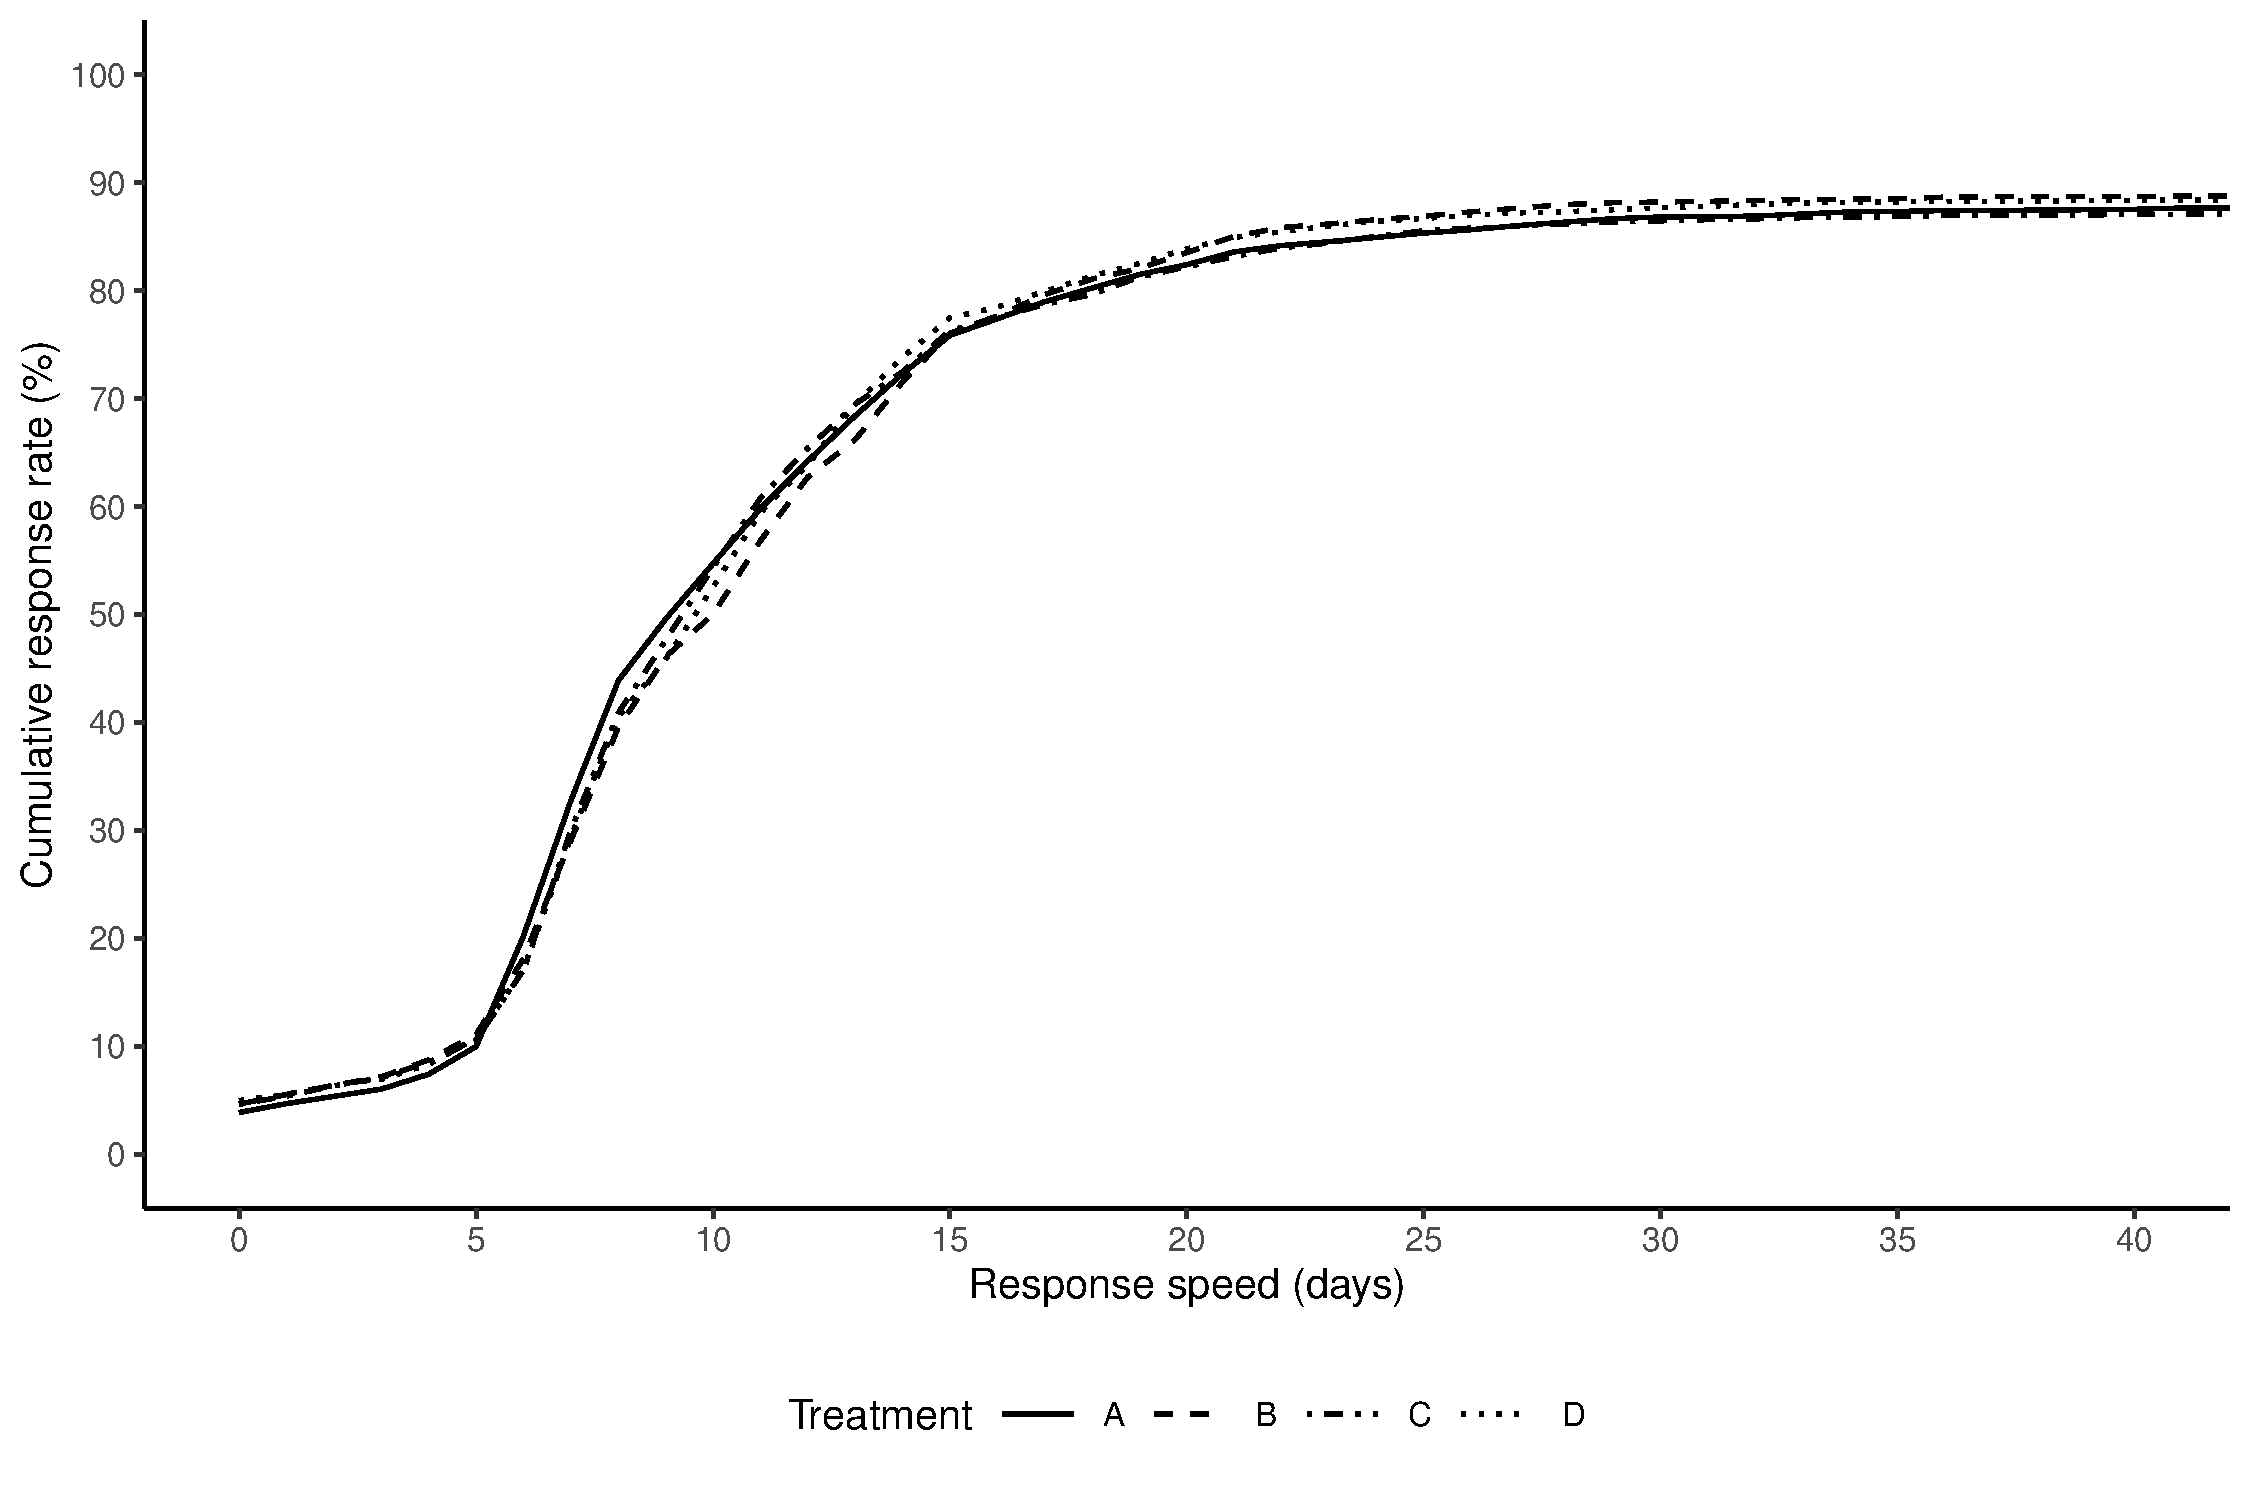
\includegraphics{JMDP RCT - Online Supplementary Material (cluster se)_files/figure-latex/cumulative-response-rate-1} \caption{Cumulative Response Rates by Treatments}\label{fig:cumulative-response-rate}
\end{figure}

\begin{figure}[H]
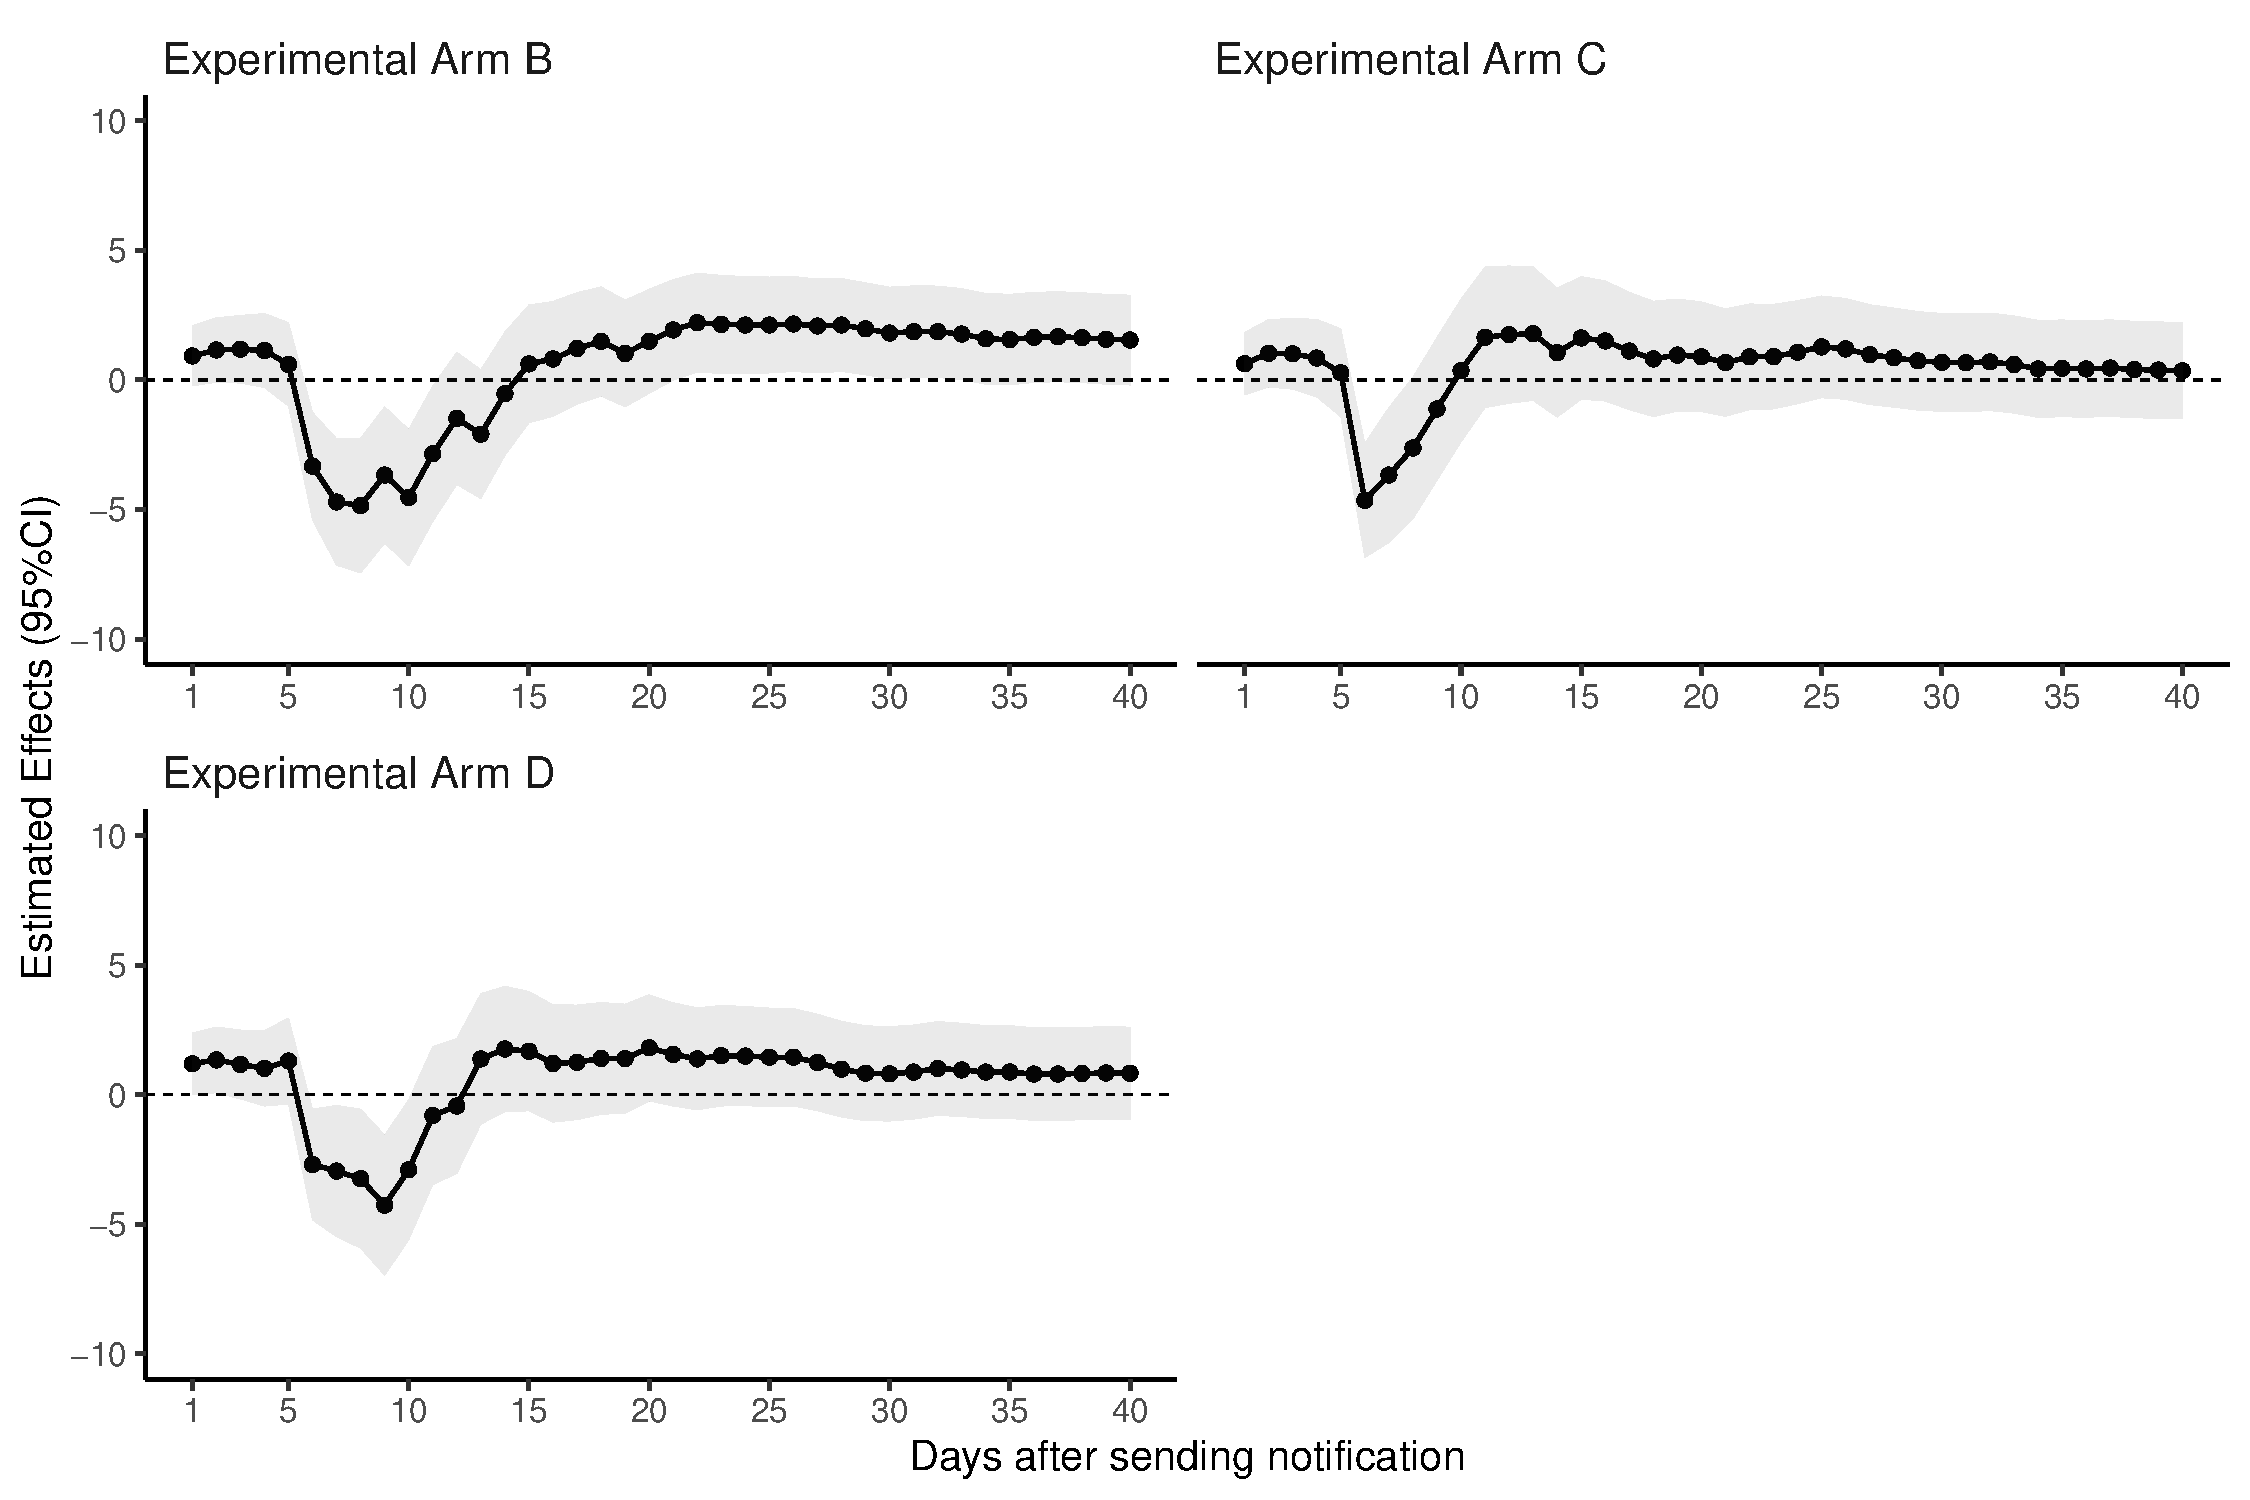
\includegraphics{JMDP RCT - Online Supplementary Material (cluster se)_files/figure-latex/flow-1} \caption{Effect on Response Speed. \newline \emph{Note}: These plots show the difference in cumulative responses on a specific day between the treated and the control arm (and the associated 95 percent confidence interval). The unit of treatment effect is a percentage point. Additionally, we used robust standard errors. We controlled for the number of past coordinations, the number of hospitals per 10 square kilometers, the number of hospitals with PBSC collection per 10 square kilometers, the number of hospitals with BM collection per 10 square kilometers, month dummies, and week dummies.}\label{fig:flow}
\end{figure}

\begin{figure}[H]
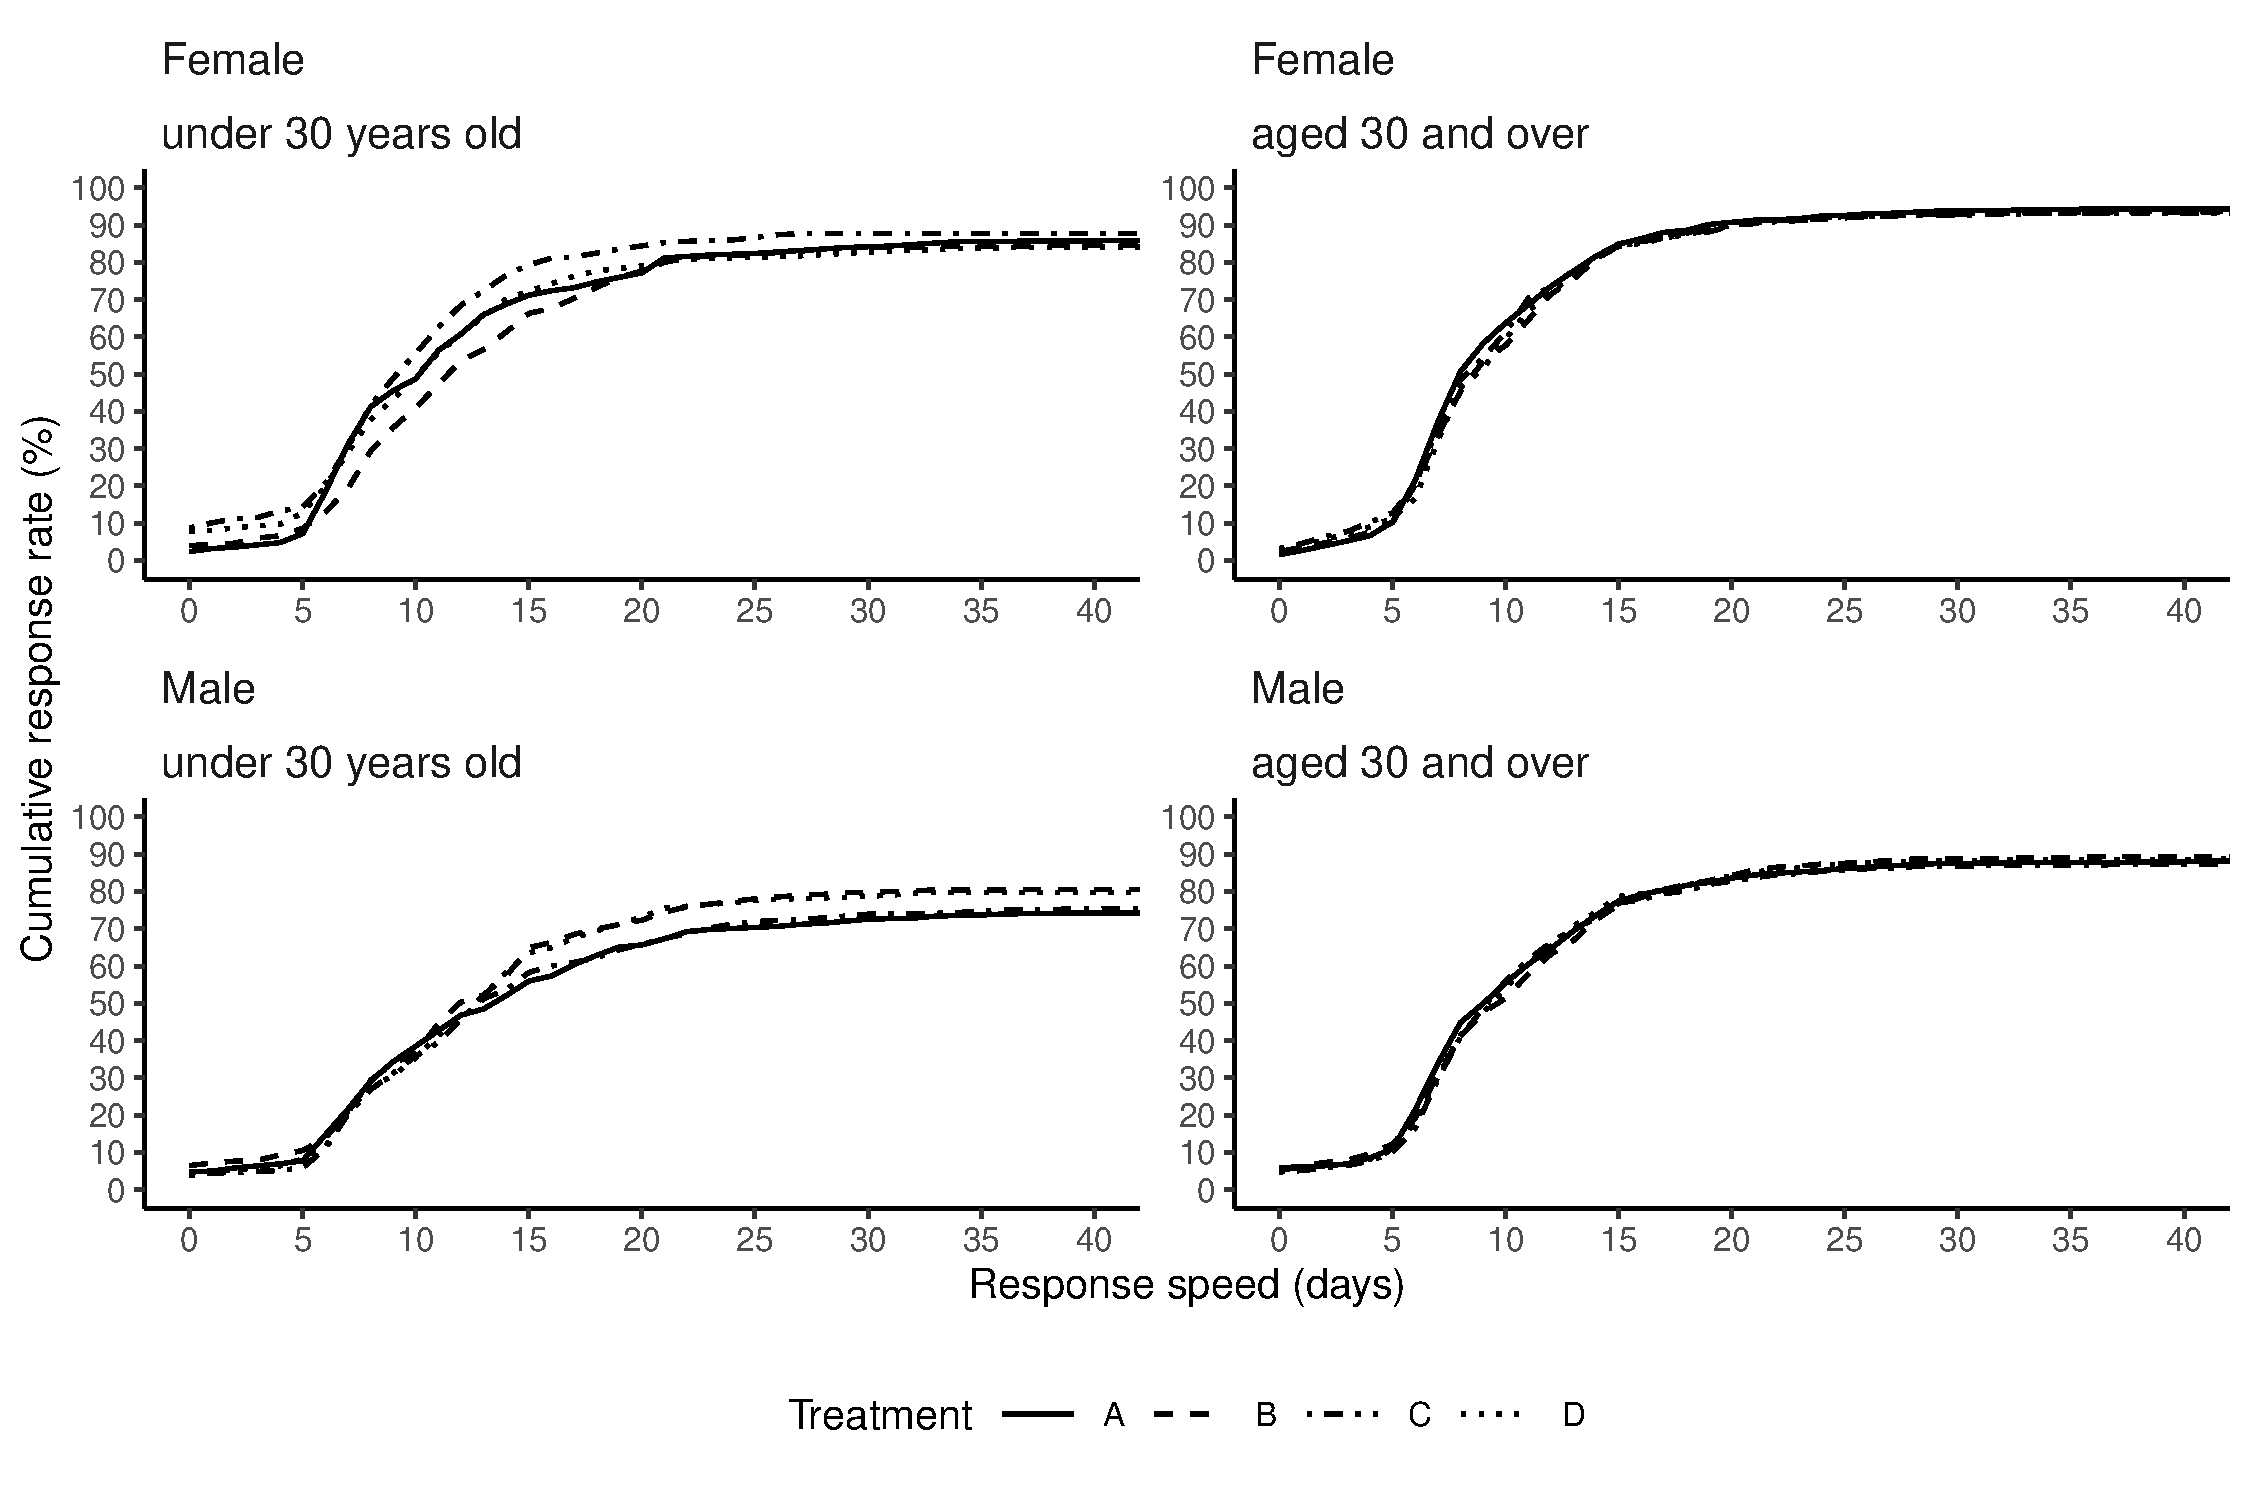
\includegraphics{JMDP RCT - Online Supplementary Material (cluster se)_files/figure-latex/cumulative-response-rate-subset-1} \caption{Cumulative Response Rates by Treatments, Gender and Age Group (Age Cutoff: 30).}\label{fig:cumulative-response-rate-subset}
\end{figure}

\begin{figure}[H]
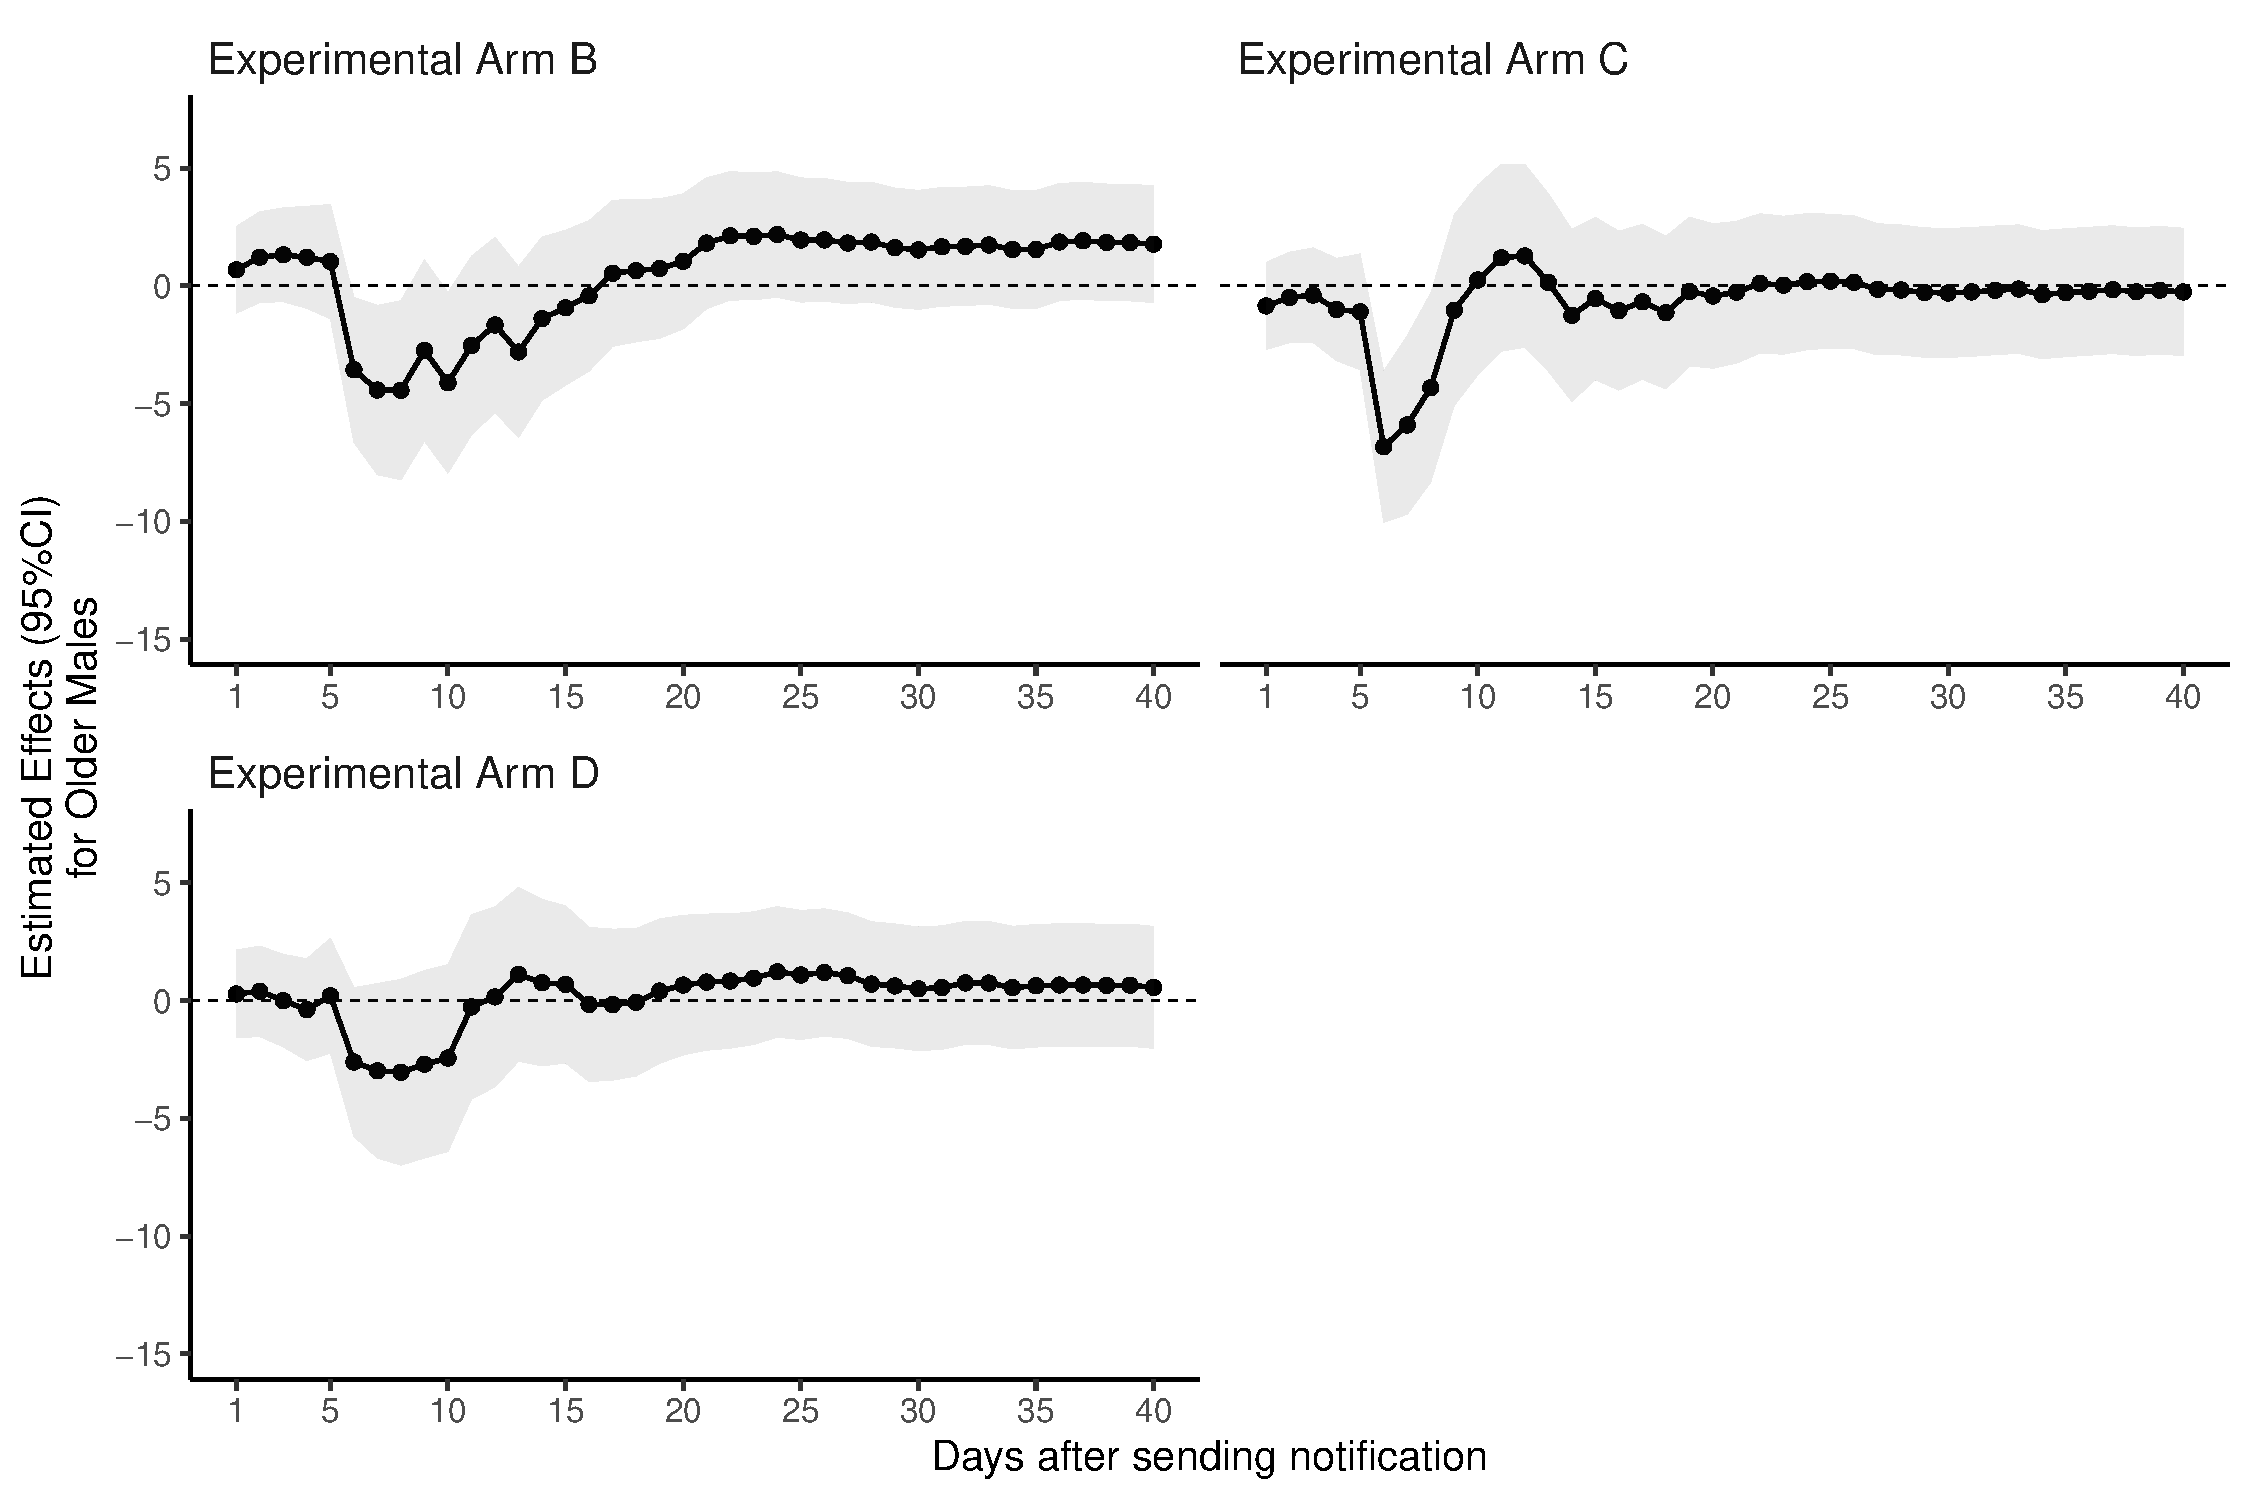
\includegraphics{JMDP RCT - Online Supplementary Material (cluster se)_files/figure-latex/old-male-flow-1} \caption{Effect on Response Speed of Older Males.\newline \emph{Note}: These plots show the difference in cumulative responses on a specific day between the treated and the control arm (and the associated 95 percent confidence interval). The unit of the treatment effect is a percentage point. We used males older than 30 for the analysis sample. Furthermore,  we used robust standard errors. We controlled for the number of past coordinations, the number of hospitals per 10 square kilometers, the number of hospitals with PBSC collection per 10 square kilometers, the number of hospitals with BM collection per 10 square kilometers, month dummies, and week dummies.}\label{fig:old-male-flow}
\end{figure}

\begin{figure}[H]
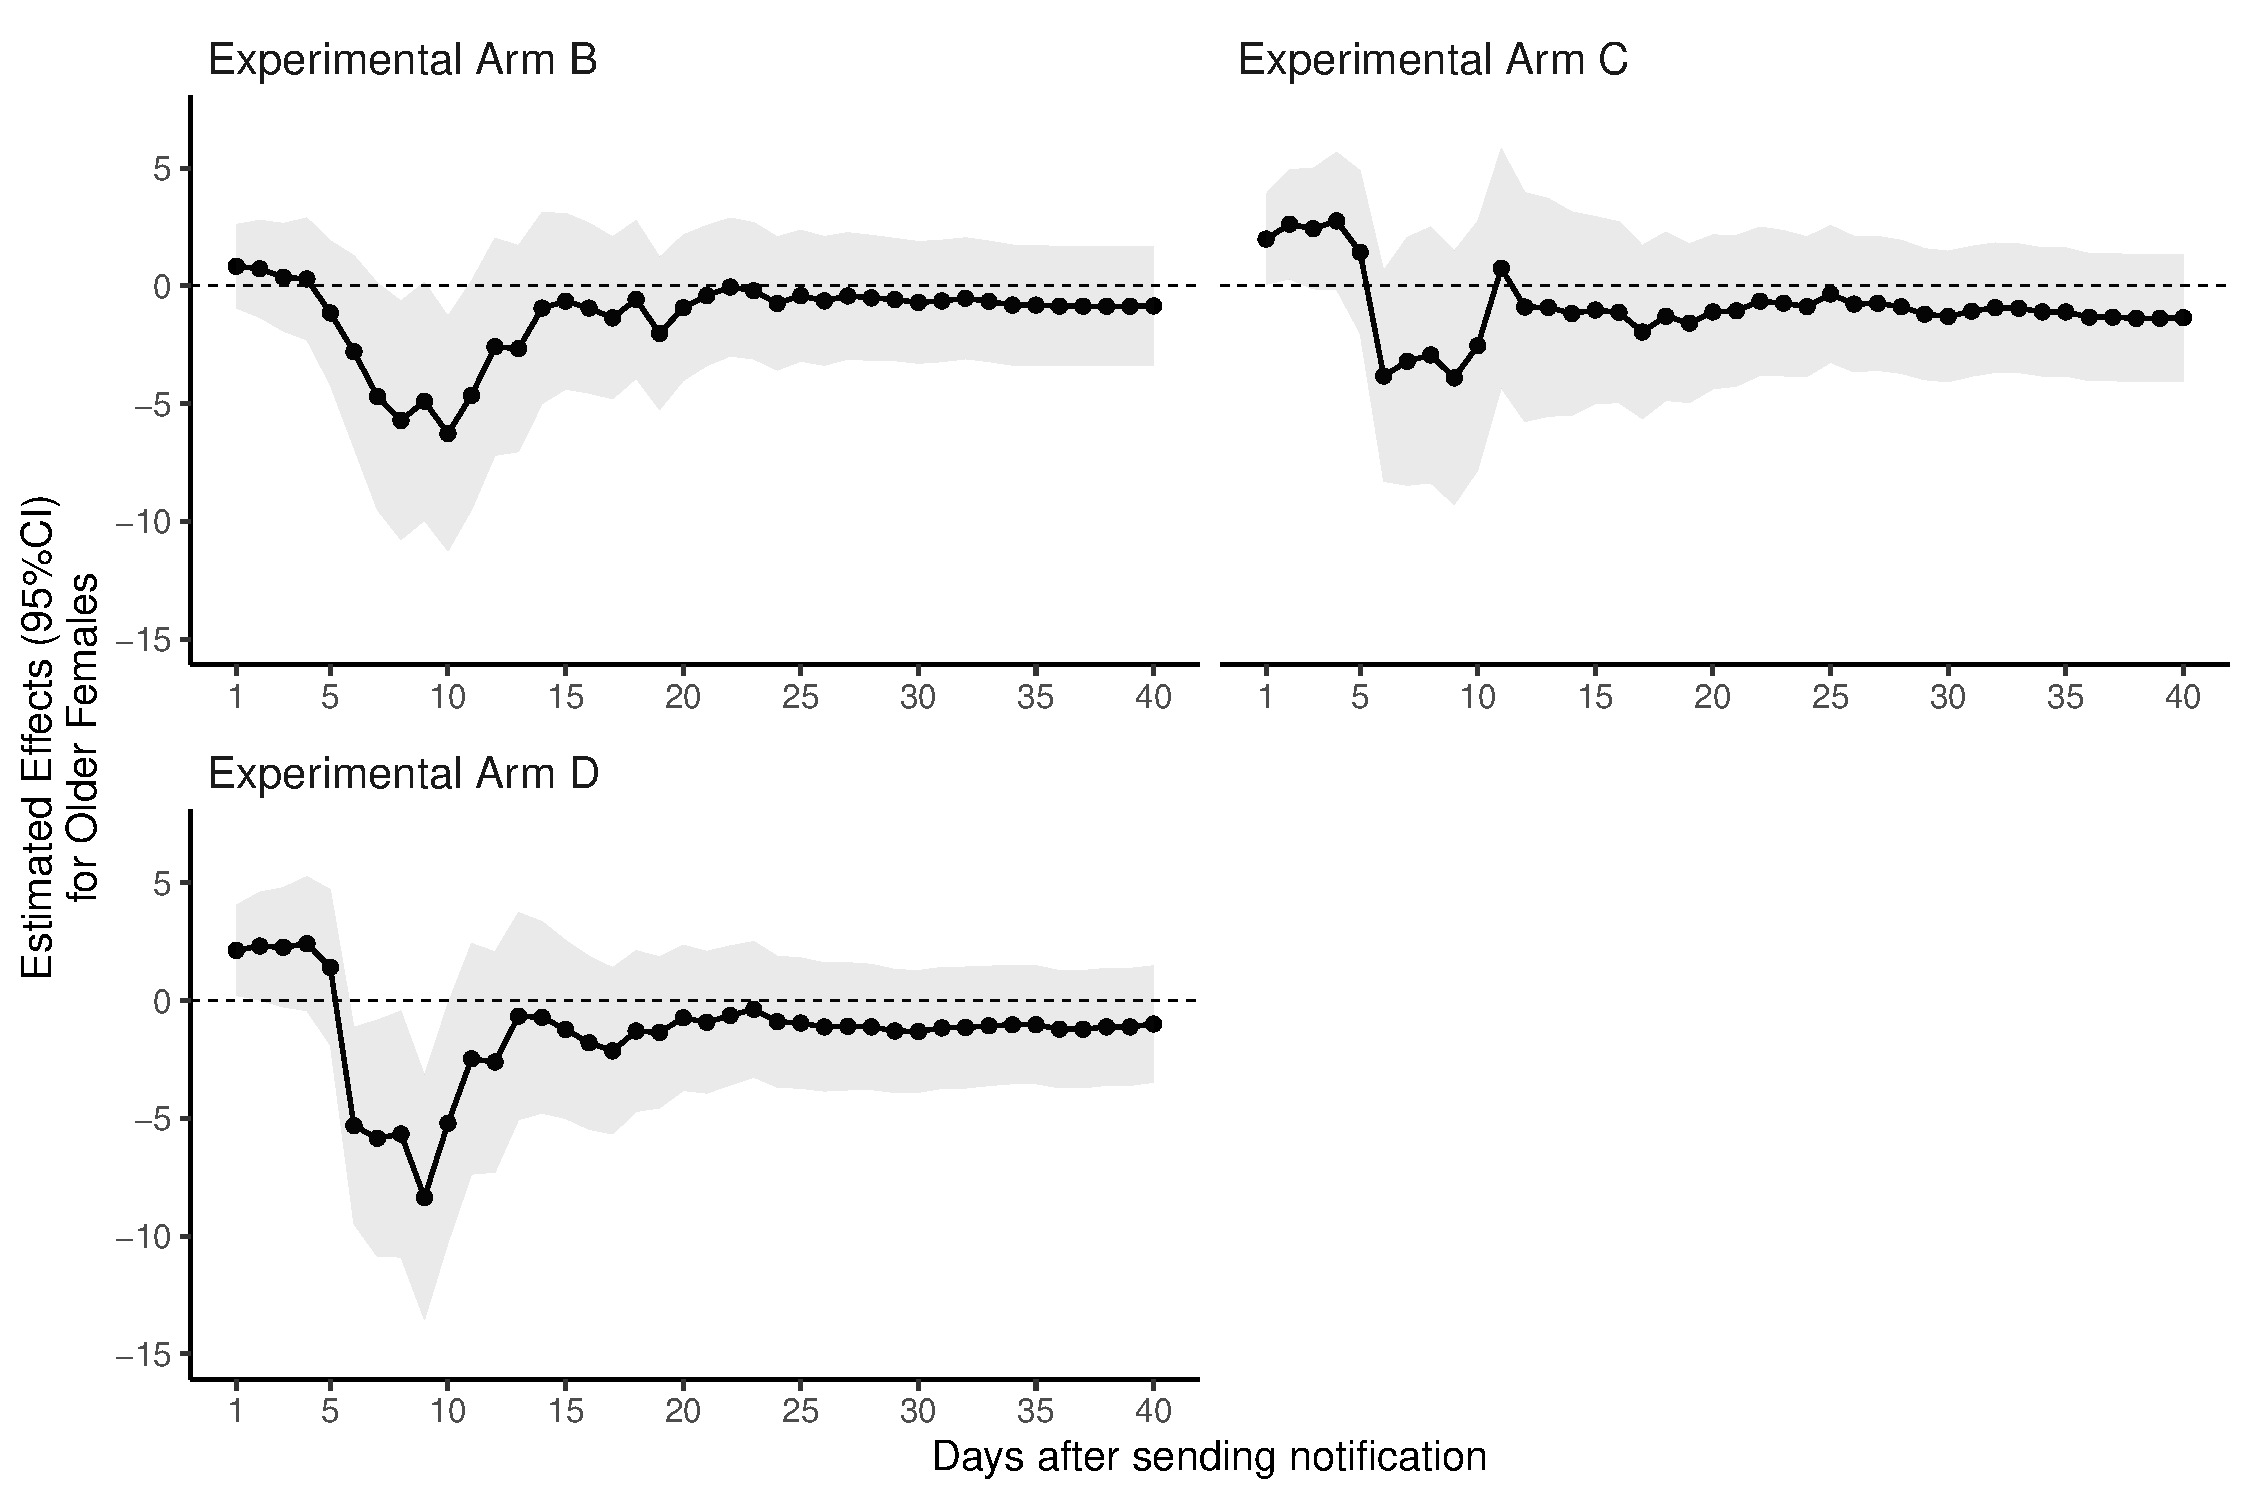
\includegraphics{JMDP RCT - Online Supplementary Material (cluster se)_files/figure-latex/old-female-flow-1} \caption{Effect on Response Speed of Older Females.\newline \emph{Note}: These plots show the difference in cumulative responses on a specific day between the treated and the control arm (and the associated 95 percent confidence interval). The unit of the treatment effect is a percentage point. We used females over 30 for the analysis sample. Moreover, we used robust standard errors. We controlled for the number of past coordinations, the number of hospitals per 10 square kilometers, the number of hospitals with PBSC collection per 10 square kilometers, the number of hospitals with BM collection per 10 square kilometers, month dummies, and week dummies.}\label{fig:old-female-flow}
\end{figure}

\begin{table}[H]

\caption{\label{tab:coordinate-reg}Linear Probability Model of Coordination}
\centering
\fontsize{9}{11}\selectfont
\begin{threeparttable}
\begin{tabular}[t]{lcccccc}
\toprule
\multicolumn{1}{c}{ } & \multicolumn{2}{c}{Candidate selection} & \multicolumn{2}{c}{Final consent} & \multicolumn{2}{c}{Donation} \\
\cmidrule(l{3pt}r{3pt}){2-3} \cmidrule(l{3pt}r{3pt}){4-5} \cmidrule(l{3pt}r{3pt}){6-7}
  & (1) & (2) & (3) & (4) & (5) & (6)\\
\midrule
Treatment B & \num{0.16} & \num{-0.06} & \num{0.26} & \num{0.01} & \num{0.12} & \num{-0.10}\\
 & (\num{0.59}) & (\num{0.40}) & (\num{0.56}) & (\num{0.34}) & (\num{0.45}) & (\num{0.36})\\
Treatment C & \num{-0.07} & \num{-0.34} & \num{0.06} & \num{-0.23} & \num{0.02} & \num{-0.25}\\
 & (\num{0.76}) & (\num{0.41}) & (\num{0.64}) & (\num{0.32}) & (\num{0.57}) & (\num{0.35})\\
Treatment D & \num{0.50} & \num{0.49} & \num{0.63} & \num{0.59} & \num{0.07} & \num{0.03}\\
 & (\num{0.72}) & (\num{0.35}) & (\num{0.80}) & (\num{0.39}) & (\num{0.74}) & (\num{0.43})\\
\midrule
Control average & 6.19 & 6.19 & 5.44 & 5.44 & 4.50 & 4.50\\
Covariates &  & X &  & X &  & X\\
Num.Obs. & \num{11049} & \num{11049} & \num{11049} & \num{11049} & \num{11049} & \num{11049}\\
\bottomrule
\multicolumn{7}{l}{\rule{0pt}{1em}* p $<$ 0.1, ** p $<$ 0.05, *** p $<$ 0.01}\\
\end{tabular}
\begin{tablenotes}
\item \emph{Note}: * $p < 0.1$, ** $p < 0.05$, *** $p < 0.01$. The robust standard errors are in parentheses. The unit of treatment effect is a percentage point. Covariates are gender, (demeaned) age, its squared term, the number of past coordinations, the number of hospitals per 10 square kilometers, the number of hospitals with PBSC collection per 10 square kilometers, the number of hospitals with BM collection per 10 square kilometers, month dummies, and week dummies.
\end{tablenotes}
\end{threeparttable}
\end{table}

\begin{table}[H]

\caption{\label{tab:coordinate-logit}Logit Model of Coordination}
\centering
\fontsize{9}{11}\selectfont
\begin{threeparttable}
\begin{tabular}[t]{lcccccc}
\toprule
\multicolumn{1}{c}{ } & \multicolumn{2}{c}{Candidate selection} & \multicolumn{2}{c}{Final consent} & \multicolumn{2}{c}{Donation} \\
\cmidrule(l{3pt}r{3pt}){2-3} \cmidrule(l{3pt}r{3pt}){4-5} \cmidrule(l{3pt}r{3pt}){6-7}
  & (1) & (2) & (3) & (4) & (5) & (6)\\
\midrule
Treatment B & \num{1.03} & \num{0.99} & \num{1.05} & \num{1.00} & \num{1.03} & \num{0.97}\\
 & {}[\num{0.83}, \num{1.28}] & {}[\num{0.79}, \num{1.24}] & {}[\num{0.83}, \num{1.32}] & {}[\num{0.79}, \num{1.27}] & {}[\num{0.80}, \num{1.32}] & {}[\num{0.75}, \num{1.27}]\\
Treatment C & \num{0.99} & \num{0.94} & \num{1.01} & \num{0.96} & \num{1.00} & \num{0.95}\\
 & {}[\num{0.79}, \num{1.24}] & {}[\num{0.74}, \num{1.19}] & {}[\num{0.80}, \num{1.28}] & {}[\num{0.75}, \num{1.24}] & {}[\num{0.77}, \num{1.30}] & {}[\num{0.72}, \num{1.25}]\\
Treatment D & \num{1.09} & \num{1.09} & \num{1.12} & \num{1.12} & \num{1.02} & \num{1.01}\\
 & {}[\num{0.87}, \num{1.35}] & {}[\num{0.86}, \num{1.36}] & {}[\num{0.89}, \num{1.42}] & {}[\num{0.88}, \num{1.42}] & {}[\num{0.78}, \num{1.32}] & {}[\num{0.77}, \num{1.32}]\\
\midrule
Covariates &  & X &  & X &  & X\\
Num.Obs. & \num{11049} & \num{11049} & \num{11049} & \num{11049} & \num{11049} & \num{11049}\\
Log.Lik. & \num{-2610.914} & \num{-2548.022} & \num{-2410.035} & \num{-2348.250} & \num{-2045.363} & \num{-2001.995}\\
\bottomrule
\multicolumn{7}{l}{\rule{0pt}{1em}* p $<$ 0.1, ** p $<$ 0.05, *** p $<$ 0.01}\\
\end{tabular}
\begin{tablenotes}
\item \emph{Note}: We show odds ratios and associated 95 percent confidential intervals in square brackets. We show odds ratios and associated 95 percent confidence intervals in square brackets. Covariates are gender, (demeaned) age, its squared term, the number of past coordinations, the number of hospitals per 10 square kilometers, the number of hospitals with PBSC collection per 10 square kilometers, the number of hospitals with BM collection per 10 square kilometers, month dummies, and week dummies.
\end{tablenotes}
\end{threeparttable}
\end{table}

\begin{table}[H]

\caption{\label{tab:coordinate-reg-subset-2}Subsample Analysis for Coordination Process (Age Cutoff: 40)}
\centering
\begin{threeparttable}
\fontsize{9}{11}\selectfont
\begin{tabular}[t]{lccc}
\toprule
 & Candidate selection & Final consent & Donation\\
\midrule
\addlinespace[0.3em]
\multicolumn{4}{l}{\textbf{Young females (N = 2268)}}\\
\hspace{1em}Treatment B & -1.71*** (0.48) & -1.74*** (0.53) & -0.87** (0.44)\\
\hspace{1em}Treatment C & 1.12** (0.54) & 0.97* (0.49) & 0.84 (0.52)\\
\hspace{1em}Treatment D & -0.34 (0.45) & -0.67 (0.49) & -0.56 (0.52)\\
\hspace{1em}Control average & 4.88 & 4.27 & 3.46\\
\addlinespace[0.3em]
\multicolumn{4}{l}{\textbf{Older females (N = 1882)}}\\
\hspace{1em}Treatment B & -0.71 (0.58) & -0.02 (0.58) & -0.16 (0.59)\\
\hspace{1em}Treatment C & -0.82 (0.56) & -0.22 (0.59) & -0.62 (0.48)\\
\hspace{1em}Treatment D & 0.33 (0.77) & 0.71 (0.63) & -0.24 (0.56)\\
\hspace{1em}Control average & 3.90 & 3.03 & 2.81\\
\addlinespace[0.3em]
\multicolumn{4}{l}{\textbf{Young males (N = 3445)}}\\
\hspace{1em}Treatment B & 0.96 (0.91) & 0.69 (0.65) & 0.48 (0.60)\\
\hspace{1em}Treatment C & -1.21 (1.04) & -1.33 (0.83) & -0.73 (0.70)\\
\hspace{1em}Treatment D & -0.07 (0.78) & 0.36 (0.70) & -0.24 (0.70)\\
\hspace{1em}Control average & 8.23 & 7.29 & 5.94\\
\addlinespace[0.3em]
\multicolumn{4}{l}{\textbf{Older males (N = 3454)}}\\
\hspace{1em}Treatment B & 0.40 (0.87) & 0.47 (0.90) & -0.18 (0.91)\\
\hspace{1em}Treatment C & 0.02 (0.99) & 0.15 (1.02) & -0.30 (1.03)\\
\hspace{1em}Treatment D & 1.72 (1.06) & 1.61 (1.12) & 0.80 (1.07)\\
\hspace{1em}Control average & 6.43 & 5.83 & 4.76\\
\bottomrule
\end{tabular}
\begin{tablenotes}
\item \emph{Note}: * $p < 0.1$, ** $p < 0.05$, *** $p < 0.01$. The robust standard errors are in parentheses. The unit of the treatment effect is a percentage point. The age category is defined as under 40 years old or older. We controlled for the number of past coordinations, the number of hospitals per 10 square kilometers, the number of hospitals with PBSC collection per 10 square kilometers, the number of hospitals with BM collection per 10 square kilometers, month dummies, and week dummies.
\end{tablenotes}
\end{threeparttable}
\end{table}

\clearpage

\bibliography{biblio.bib}



\end{document}
